
\documentclass{article}
\usepackage{graphicx}
\title{Reinforcement learning\\ Homework 2\\ Alexandru Dumitrescu}
\date{}
\begin{document}
\maketitle
\section{Question 1}
The agent is the sailor and the enviornment is the sea (and everything it contains: rocks, winds - with random movement probabilities, calm water - with the other random movement probabilities and the harbour).

\section{Question 2}
The value function represents the expected discounted future rewards, therefore, in a final state, there are no future rewards and the value function is 0 for that.


\section{Question 3}
The sailor chooses the path between the two lines of rocks. If the penalty for hitting the rock is changed to -10, then the sailor will choose to go below them, as shown in the following two action-figures.\\

\centerline{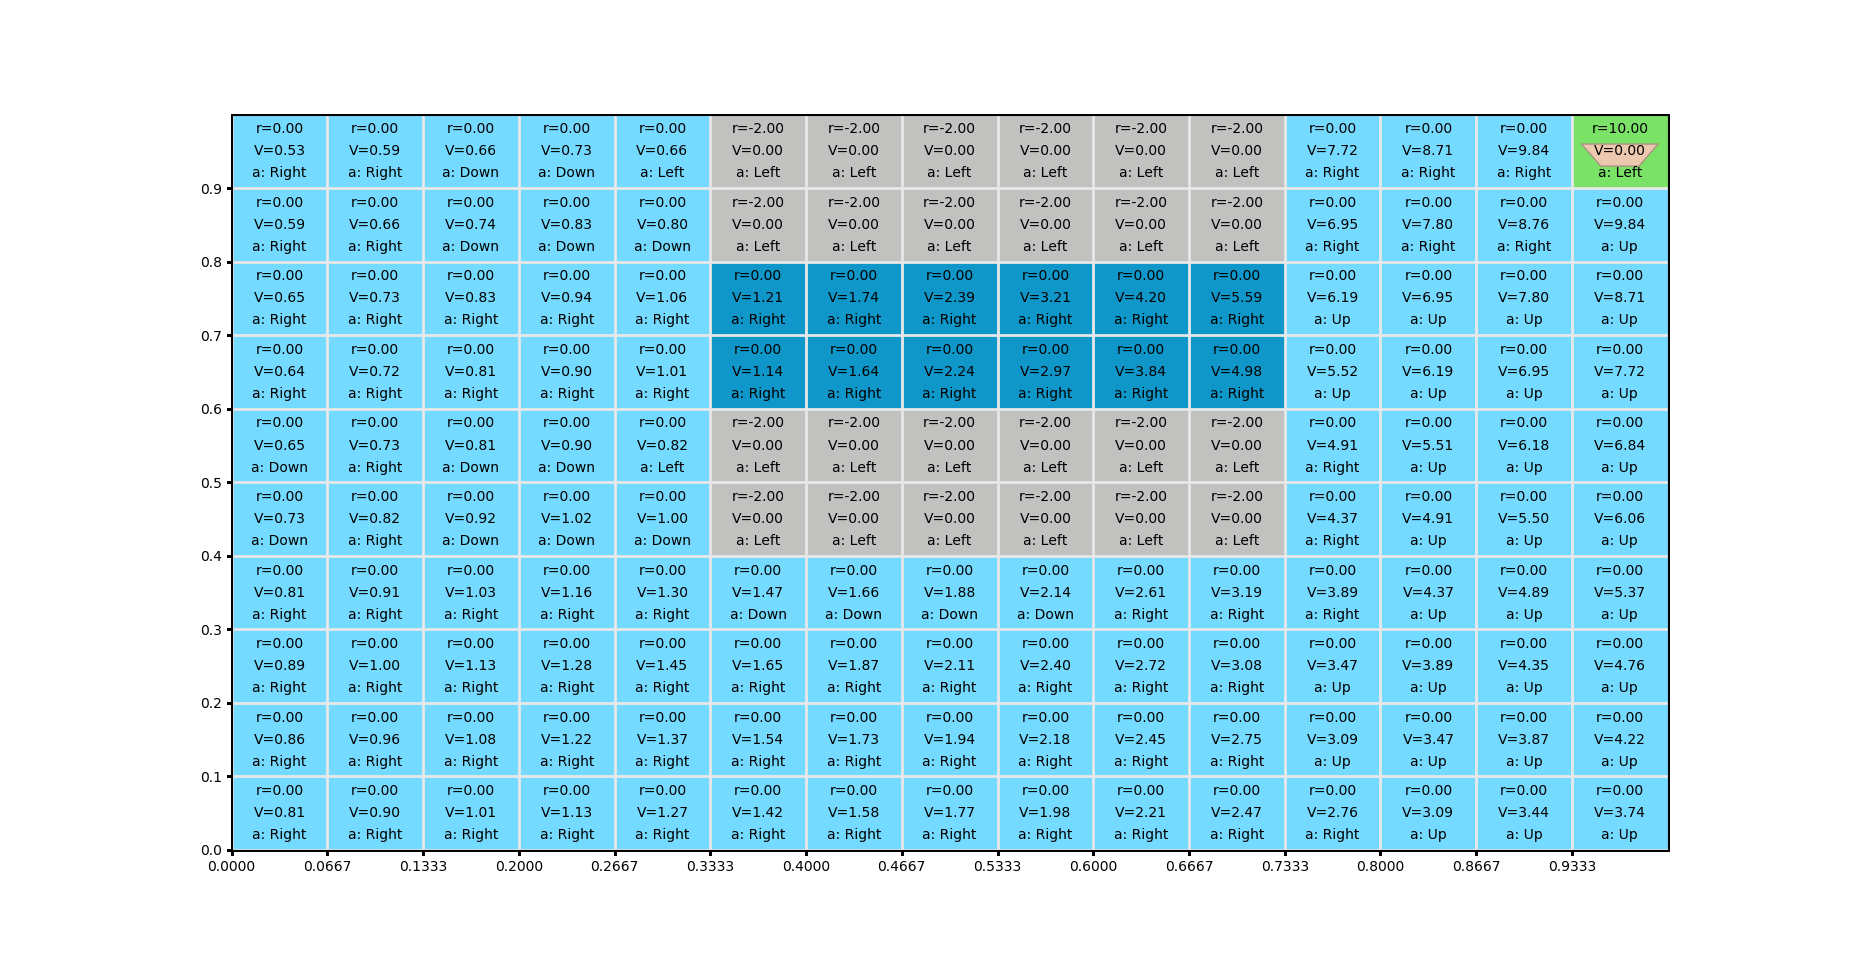
\includegraphics[scale=0.39]{Sailor_win.png}} 

\centerline{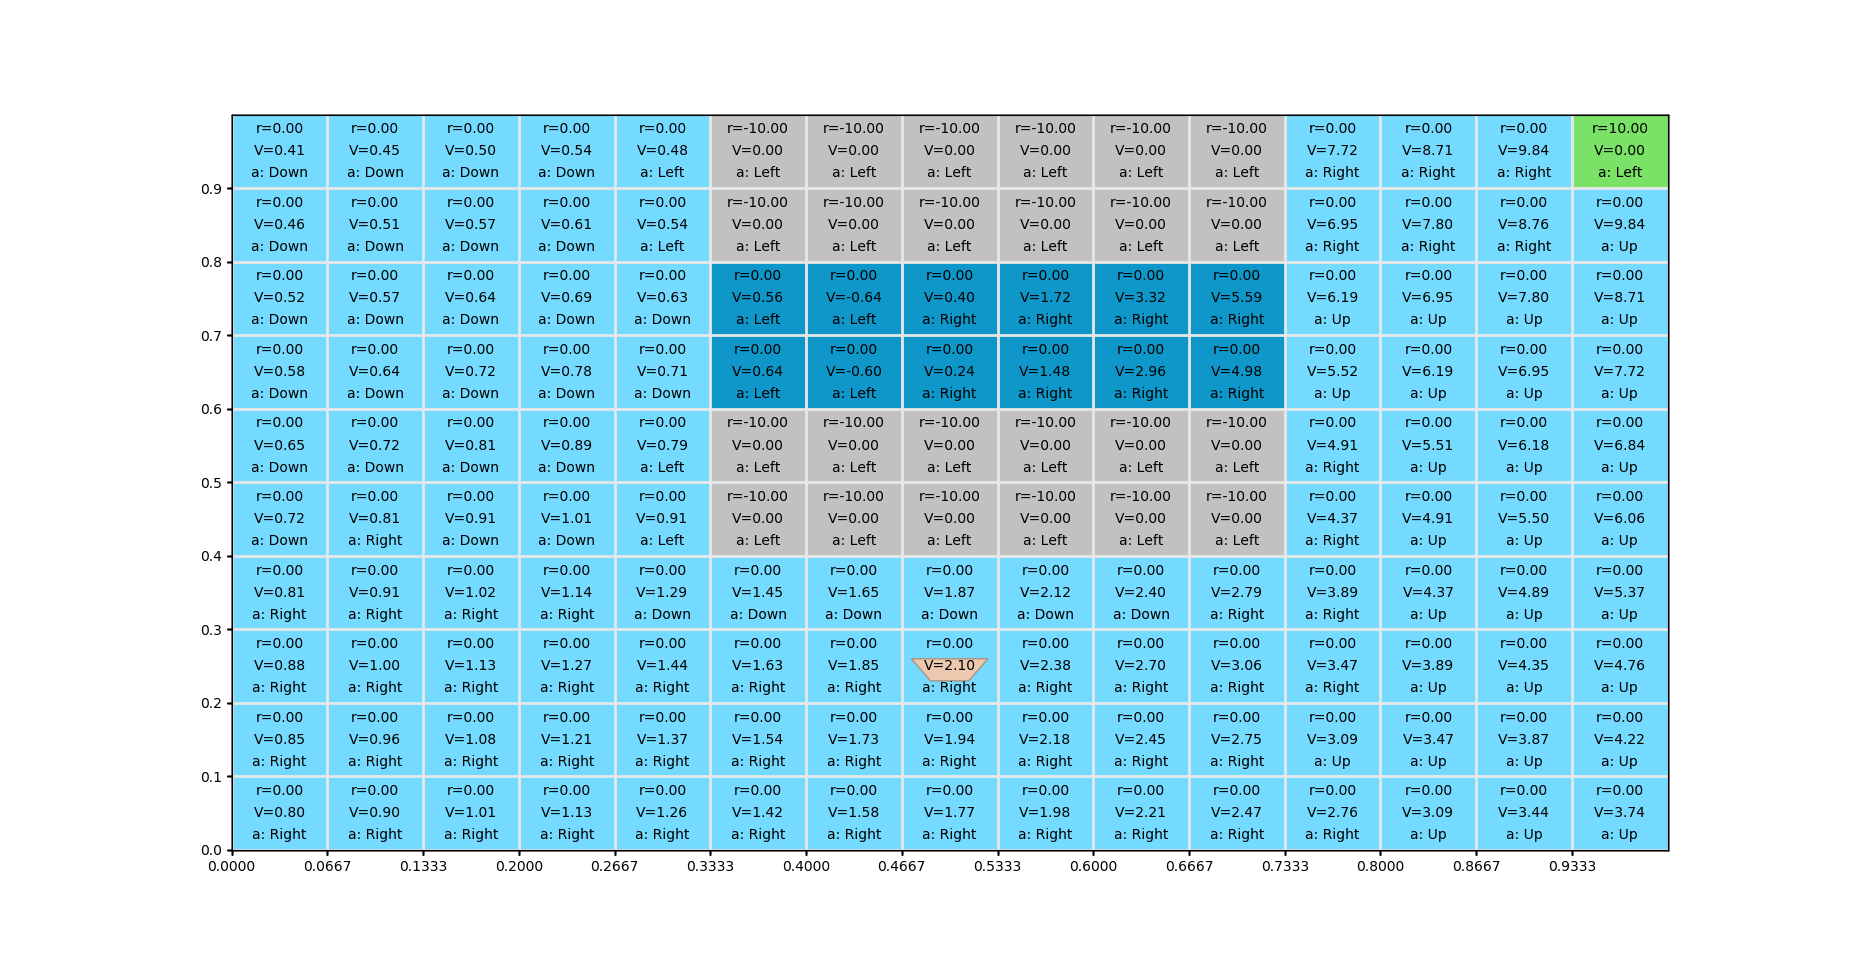
\includegraphics[scale=0.39]{below1.png}} 

\section{Question 4}

It depends how small the number of iteration is. It can be lowered and still converge, but too low (e.g. 20) does not allow the values to flow all the way from top-right to bottom-left. Other than that, it is only a matter of how we are definig convergence (what is the acceptable error - since the exact values of the optimal value function are obtained only as the number of iterations go to infinity).

 Of course, the value function must converge - we can take care on \textbf{the last iteration} to also retain which action gives the value function that maximum discounted future reward.

Another way to put it would be that the policy converges along with the value function, but the value function is the one which should converge for the policy to be optimal.

\section{Question 5}
The mean and standard deviation of 1000 returns are: $\mu = 0.63, \sigma=1.36$. The value of the value function for that point is $v[1,8]=0.65$.

The value function should converge to the sum of the discounted returns from any given point on the grid, as the number of iteration approaches infinity.  That is one of the reasons why the mean of the 1000 returns and the value function are not exactly the same (the value function converges only to infinity). The other one is that the true expected value of the returns for that given point (the starting point $1,8$), will also, by the definition of the expected value, converge exactly only to infinity.

\section{Question 6}

No, the value iteration approach wouldn't be possible. The value function represents a mapping from the state space to some values resembling discounted rewards. An unknown enviornment, having both the state space and the dynamics unknown, wouldn't be possible to be solved through this method. The unrealistic assumption would be an infinite number of iterations required for the algorithm to converge with any arbitrary error to the optimal value function, since the state space could be anything (e.g. continuous state space - so \textbf{not} a finite MDP).

\end{document}

